\documentclass[openright]{report}
\usepackage[utf8]{inputenc}
\usepackage[table]{xcolor}
\usepackage{fancyhdr}
\usepackage{extramarks}
\usepackage{amsmath}
\usepackage{amssymb}
\usepackage{flafter} 
\usepackage{amsthm}
\usepackage{multicol}
\usepackage{amsfonts}
\usepackage{tikz}
\usepackage[plain]{algorithm}
\usepackage{forest}
\usepackage{algpseudocode}
\usepackage{changepage}
\usepackage{siunitx}
\usepackage{wasysym}
\usepackage{mathtools}
\usepackage{titlesec}
\usepackage{indentfirst}
\usepackage{graphicx}
\usepackage{titletoc}
\usepackage{array}
\usepackage[hyphens,spaces,obeyspaces]{url}
\usepackage{tabulary}
\usepackage[labelformat=empty]{caption}
\usepackage[english]{babel}
\usepackage[nottoc]{tocbibind}
\usepackage{chngcntr}
\counterwithout{figure}{chapter}
\usepackage[T1]{fontenc}
\usepackage{listings}
\usepackage{xcolor}
\usepackage[scaled=.85]{beramono}

\newcolumntype{K}[1]{>{\centering\arraybackslash}p{#1}}

\graphicspath{ {images/} }
\usetikzlibrary{automata,positioning}

\usetikzlibrary{shapes.geometric, arrows}

\tikzstyle{startstop} = [rectangle, rounded corners, minimum width=3cm, minimum height=1cm,text centered, draw=black, fill=red!30]
\tikzstyle{io} = [trapezium, trapezium left angle=70, trapezium right angle=110, minimum width=3cm, minimum height=1cm, text centered, draw=black, fill=blue!30]
\tikzstyle{process} = [rectangle, minimum width=3cm, minimum height=1cm, text centered, text width=3cm, draw=black, fill=orange!30]
\tikzstyle{decision} = [diamond, minimum width=3cm, minimum height=1cm, text centered, draw=black, fill=green!30]
\tikzstyle{arrow} = [thick,->,>=stealth]

\renewcommand{\familydefault}{\rmdefault}

\topmargin=-0.45in
\evensidemargin=0in
\oddsidemargin=0in
\textwidth=6.5in
\textheight=9.0in

\linespread{1.25}

\pagestyle{fancy}

\renewcommand{\chaptermark}[1]{\markboth{#1}{}}

\lhead{\projectAuthorShort}
\chead{\reportTopic}
\rhead{\leftmark}
\lfoot{\lastxmark}
\cfoot{\thepage}

\newcommand{\reportTopic}{Phase I and II Report}
\newcommand{\projectAuthorShort}{Cybersecurity Education Group}
\newcommand{\projectTitle}{Hands-on Cybersecurity Education}
\newcommand{\reportDueDate}{February 23, 2018}
\newcommand{\reportClass}{Synthesis Design II}
\newcommand{\reportClassInstructor}{Professor Dana Elzey}
\newcommand{\reportAuthorName}{Clark Benham (cb5ye), Calvin Krist (czk4ja), Saeed Razavi (slr4gf),\\and Jake Smith (jts5np)}
\newcommand{\collaborators}{}

\title{
    \vspace{2in}
    \LARGE{\textbf{\projectTitle}}\\
    \vspace{0.1in}\large{\reportClass:\ \reportTopic}\\
    \vspace{0.1in}\large{\reportClassInstructor}\\
    \normalsize\vspace{0.1in}\large{Due\ on\ \reportDueDate\ at 5:00pm}
    \vspace{1.4in}
}

\author{\reportAuthorName}
\date{}

\renewcommand{\contentsname}{Table of Contents}
\titlespacing*{\chapter}{0pt}{-40pt}{40pt}

\titleformat{\chapter}
  {\Large\bfseries} % format
  {}                % label
  {0pt}             % sep
  {\huge \vspace{-0.2in}}           % before-code

\begin{document}

\maketitle

\large{\tableofcontents}

\chapter{Background}

\section{Introduction}

\par Software is ubiquitous in many countries today. Companies use software to manage user data and offer services. Consumers use it to work, relax, and learn about the world. It's used by governments to help manage elections, recognize citizen needs, and protect their sovereignty. 

\par Software is also used for malicious purposes: criminals, both organized and free-lance, use software, called `malware', to attack businesses, consumers, and governments for personal gain. Malware is also used by activists such as Anonymous to damage those they view as harmful, such as their attack against the World Trade Organization\cite{anonymous_attack}. Even governments use malware for unethical purposes: the NSA's PRSIM program was discovered to be conducting warrantless surveillance on U.S. citizens\cite{nsa_illegal}. High quality programs that costs millions to produce have been used to destroy infrastructure and attack nation states, such as Stuxnet, believed to have been made by the United States\cite{stuxnet}. Autocratic regimes, such as that in Lebanon, use malware to spy on their own people and attack political dissidents\cite{lebanon}.

\par In order to combat malicious software, a specialized security field called `cybersecurity' arose that protects software systems and responds to attacks through a variety of means. Cybersecurity professionals from Gartner, an IT research company, defined the term as "security practices related to the combination of offensive and defensive actions involving or relying upon information technology and/or operational technology environments and systems"\cite{cyber_def}. In other words, the field of cybersecurity encompasses both attacking and defending systems such as computers, networks, and databases. Due to the components of these systems, cybersecurity professionals are often also called IT security professionals. This field is taught at many Universities today, and cybersecurity professionals are in high demand from both companies and governments due to the extreme integration of software into modern society and the high value of user data.

\section{Market Need}

\par At the most superficial level, malware hurts the economy and people's lives. Cyber attacks cost the global economy \$400 billion annually, and is only increasing. This cost largely comes from stealing user data, such as credit cards and medial information, and by shutting down company infrastructure. There are thousands of such attacks world-wide: in 2016, there was over 1000 data breaches of U.S. companies alone. For example, Maersk, the shipping company, had all their computer systems infected by ransomware (malware that stops the user from doing anything until they pay a fee). This completely halted their operations for over a week as they switched back to pen-and-paper management and quickly rebuilt all their servers and databases from the ground up. This attack, which did not even target the company, cost them about \$250 million\cite{maersk}. Another example comes from 2017, when Equifax was hacked, exposing the personal data of over 160 million Americans - data that included credit card numbers, social security numbers, and more. This allows criminals to steal people's identity and conduct all types of fraud.

\par It should be noted that it's not always the economy or individuals who are hurt: political systems and entire cultures can be damaged as well. For example, Russia's hacking of the elections compromised the integrity and sovereignty of the United States\cite{russa_indicement}. The operations consisted largely of leaking DNC emails and an extensive online disinformation campaign on social media, disguising the foreign influence through special servers and long-term user accounts\cite{russa_indicement_nyt}\cite{what_russia_did}. This is a corruption of the democratic culture, and could have long term effects both nationally and internationally. 

\par Autocratic regimes, or even those with a less democratic culture than the United States, often use surveillance software (spyware) to spy on political dissidents and journalists trying to report on 'politically harmful' information. As a result, many companies sell 'security solutions' to autocratic regimes such as Ethiopia which are used to spy on their citizens\cite{ethiopia_surveillance}. Mobile devices can be turned into tools of repression, where messages one sends to others expressing dissatisfaction can be means for arrest or other forms of retaliation. Countries like Saudi Arabia own large shares in infamous cyber security companies and use their products for espionage on their own \cite{saudi_cyber}. Mexico illegally uses hacking tools to spy on activists and reporters in order to intimidate and harass them\cite{mexico_cyber}. In other words, malware is actively used to support autocratic and politically harmful practices.

\par Part of this excess of cyber attacks and malware comes from the fact that IT security professionals have to defend entire systems that have hundreds of vulnerabilities, while attackers have to find just one weak point. In other words, attacking is inherently easier than defending. However, there also aren't enough qualified cybersecurity professionals for all the businesses and governments in any country, leaving user data vulnerable to attack. 90\% of companies worldwide say they are unprepared for cyber attacks, and governments similarly have trouble. 70\% of U.S. federal IT security professionals say the government lacks qualified employees, and 86\% say they have trouble finding personal to fill spots\cite{fed_cs_jobs}. It is estimated that, by 2020, there will be 1.5 million unfilled cybersecurity jobs in the U.S., leaving the way open for user data and companies to be more vulnerable than ever\cite{why_no_cyber_classes}.

\par The direct cause of this issue can be seen in a report made by the ISACA in 2017, an international association of IT professionals. They surveyed members of their association and found that most IT security job posting just get around 5 responses, and only around 10\% of job postings get at least 20 responses. In contrast, most corporate job openings receive between 60 and 250 applicants\cite{job_survey}. This is because \textit{everyone} needs IT security professionals, and there are not enough of them to go around.

\par This problem is further compounded by the fact that few of those who even respond to cybersecurity job postings are qualified: the ISACA found in their survey that nearly half of those questioned said that one in four of respondents to their job posting are qualified. The number one reason potential hires were unqualified was a lack of hands one experience\cite{job_survey}. In other words, not only do very few people respond: an astounding proportion of respondents are un-hireable. This leaves the whole world without the necessary number of cybersecurity experts to protect them.

\section{Observations}

\section{Problem Identification}

\par Why are there so few cybersecurity job applicants and why are so few of them qualified? To begin, this is a very new field. As a result, there is no consensus as to what students should be taught and how they should be taught\cite{why_no_cyber_classes}. This means that there can be a large discrepancy between what employers want, what employers need, and what students are taught. Furthermore, not many universities offer undergraduate degrees in cybersecurity, much less a quality education in the field. This includes the University of Virginia. Here at UVA, there is currently a lot of debate between CS professors as to how much security education should be required to get a degree. Currently, while numerous security courses are offered and more are coming, there is no requirement to take one\cite{comsci_handbook}. Students only study cybersecurity if it interests them.

\par This results in two things: normal software developers leave more vulnerabilities in their applications, and less students become interested in cybersecurity. Not teaching basic security to CS undergraduates means that those students, now professional developers, are not aware of the security needs of applications or the ways that they can expose user data. This means lots of software, much of which is used by consumers, have vulnerabilities that can be abused by malicious hackers\cite{why_no_cyber_classes}. If graduates were required to take basic security courses, they may be more cognizant of the security of their applications and consumers would be safer.

\par Furthermore, many students will not take cybersecurity courses unless it is required. Cybersecurity, in contrast to most of computer science, is very intimidating. It has a dry reputation, and it's generous to say that there even \textit{basics} to cybersecurity. As we have seen by talking with students, many don't know where to begin studying the topic. 

\par Cybersecurity requires vast domain experience due to the diversity of systems that need to be protected. As a result, it's hard to learn and hard to become passionate about because there is no immediate payoff to studying it. This means that few students will become interested in the field on their own, and without universities pushing students towards towards the field, this problem will not be rectified.

\par Even for those who decide cybersecurity is a topic worth pursuing, there are many barriers. Much of cybersecurity is about the interaction of systems. This means that to do more than read about topics--to get hands on experience--students need to be able to set up or simulate the systems they read about. Students need to know more than just intermediate programming and network theory: they also need to be server experts, OS experts, and knowledgeable about service architecture. 

\par This asks a lot of students. The necessary complexity of these systems makes them difficult to set up, and even following an online tutorial is frustrating. Small differences in computer configurations can result in hours of hard work debugging the problem. This is very discouraging, and can slow down student learning or even dissuade them from the field entirely. 

\par These same problems are why many university graduates lack hands on experience and are unqualified for most IT security jobs. Because of the nature of teaching in a classroom, the labs have to work for all students. If the lab doesn't work on one student's computer, the professor is faced with a painful decision: to leave the student behind, or hold up the whole class to try and debug the issue. As a result, most labs are as simple as possible while still demonstrating core concepts to reduce the time spent setting up and the risk of a student not being able to participate\cite{ibrahiminterview}. This means that, for universities to give students hands on experience, the best technology right now is to have dedicated computer labs set up for students to use. A computer for every student, enough routers and servers for all of them, the databases necessary. This would be incredibly expensive, take lots of time to set up, test, and prepare, and it still could fail.

\par The result is that schools can't give students hands on experience and students have lots of trouble getting that experience themselves. Thus, most of those that do choose to study this field lack the requisite experience necessary to be a qualified IT security professional.

\begin{center}
    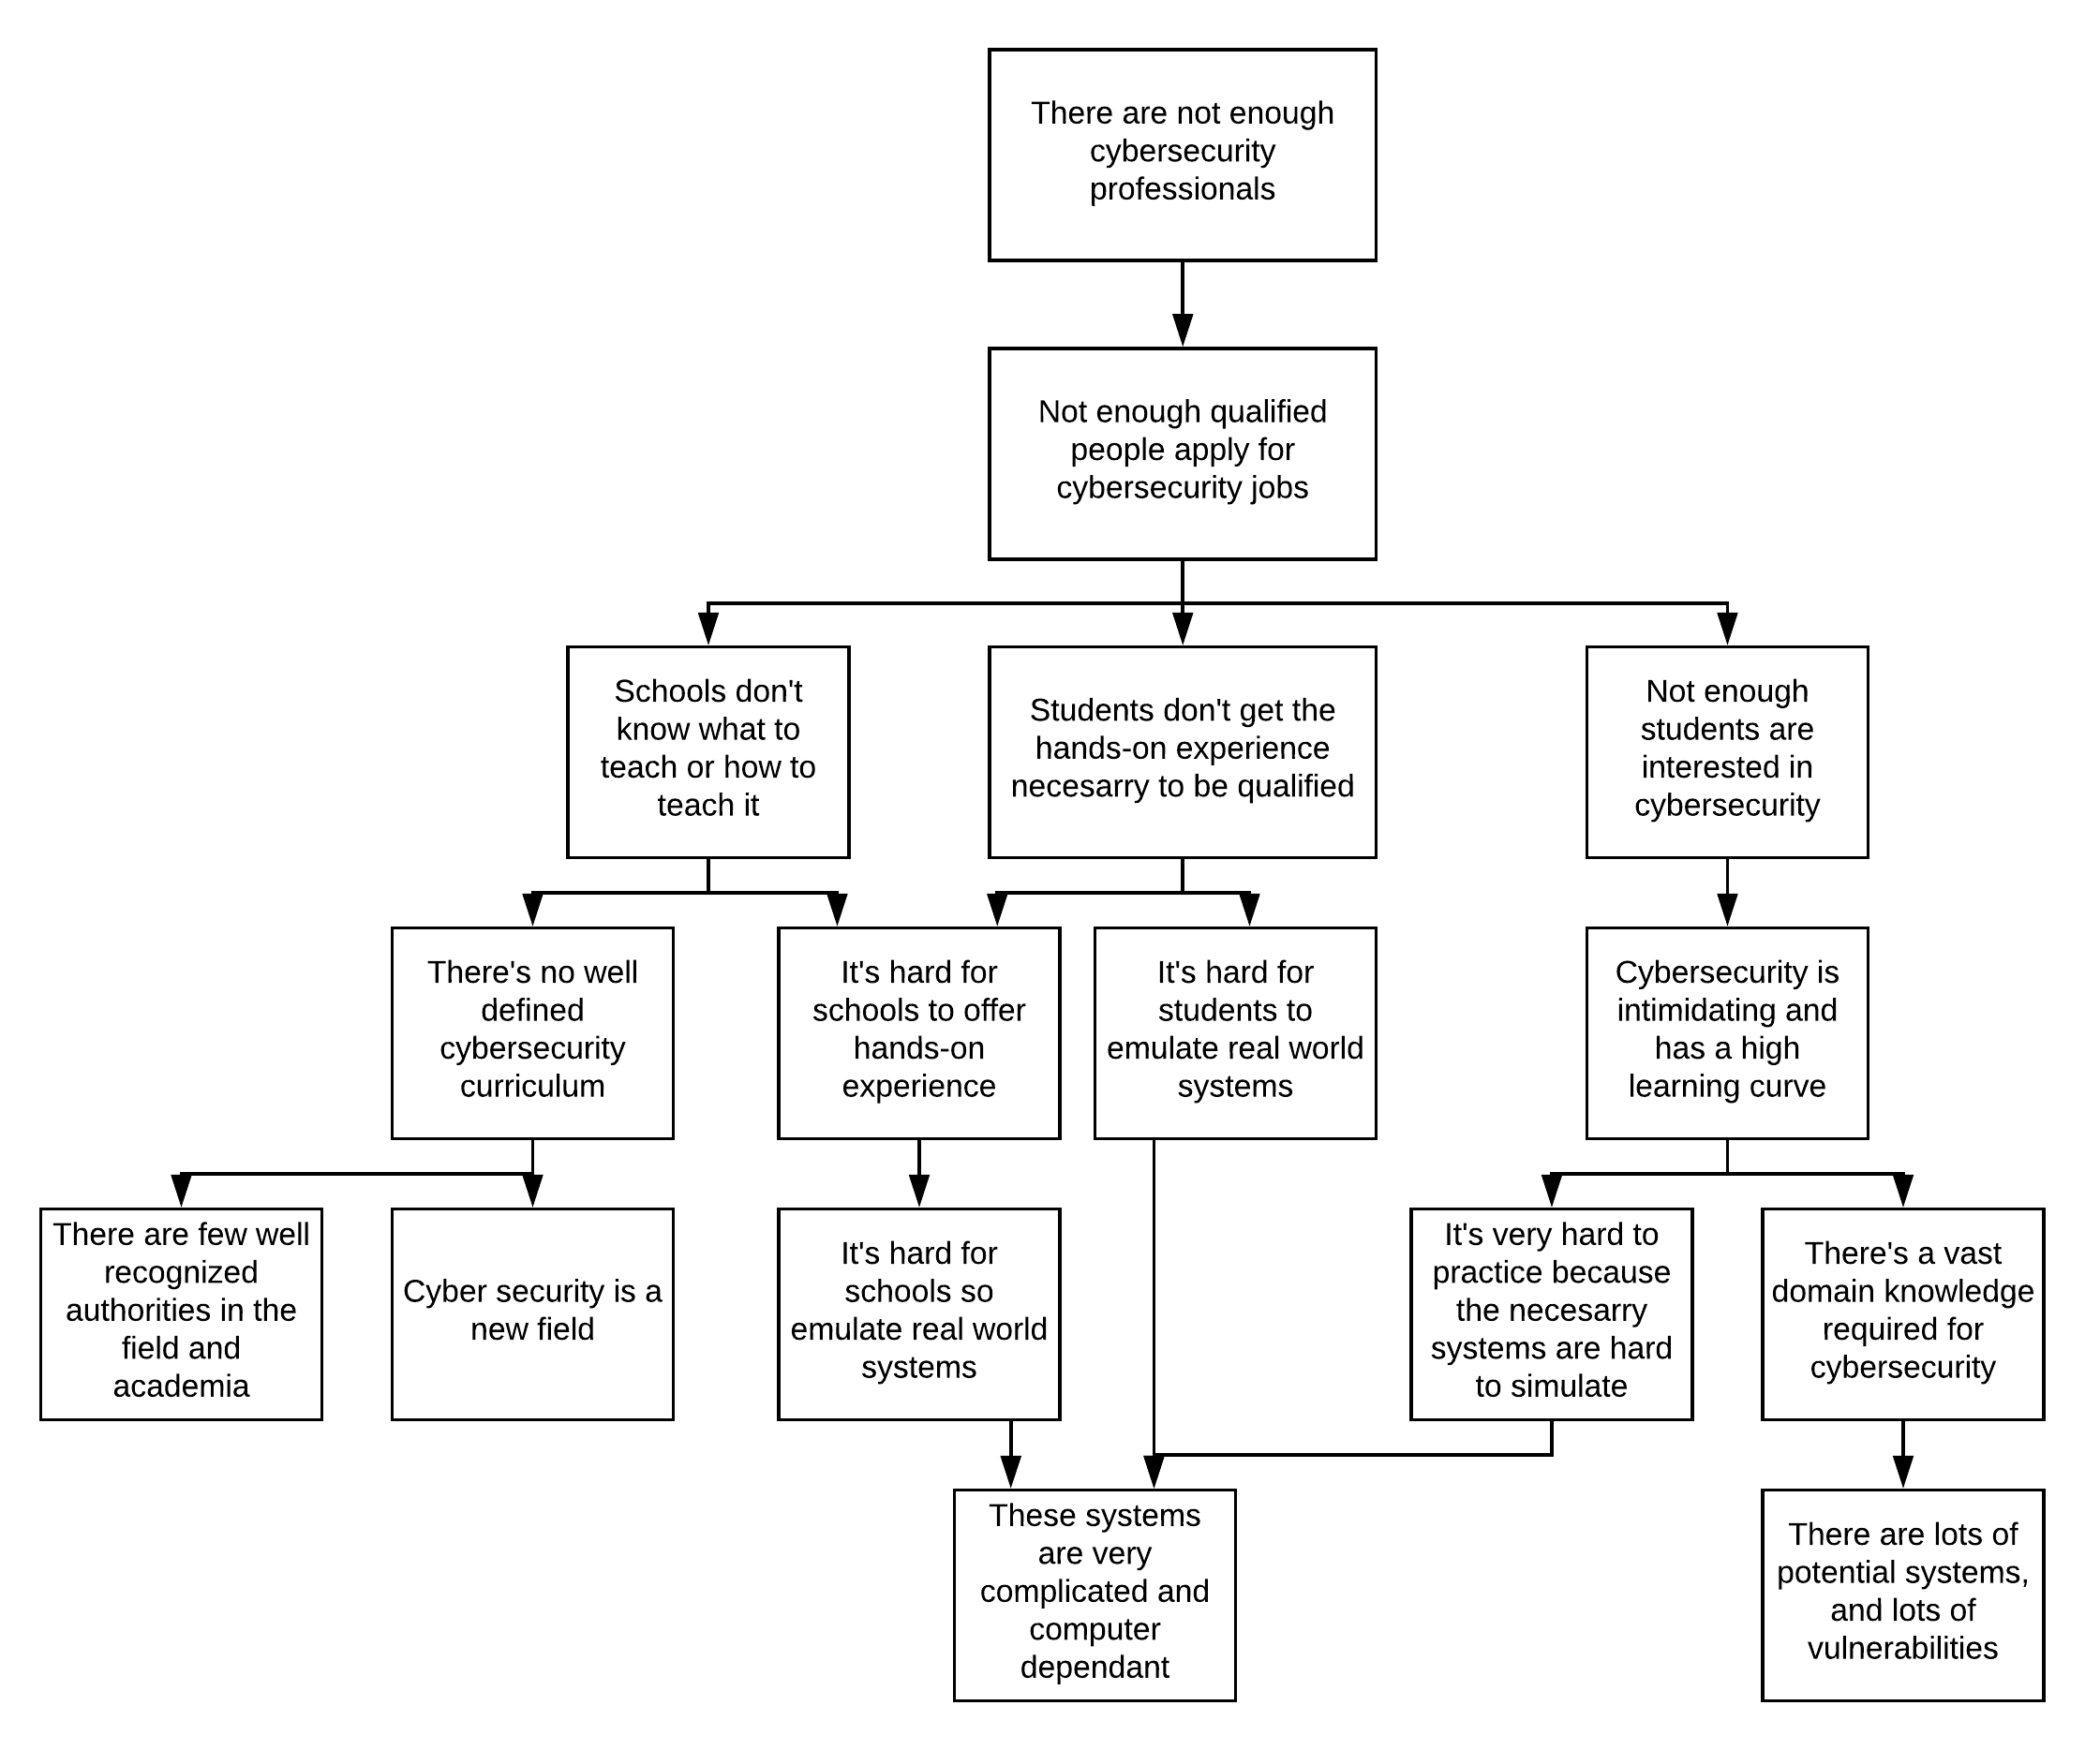
\includegraphics[scale=0.34]{images/Why-Why.png}
    \captionof{figure}{\textbf{Figure \arabic{figure}:} Why-Why Diagram identifying the problem}
\end{center}

\par As can be seen in Figure 1, there are a few different conclusions that can be drawn. As has been discussed, cybersecurity is complicated because the systems it needs to defend are complicated: that can't be changed because the systems serve users. Furthermore, the line of inquiry regarding curricula is currently being worked on by other entities with lots of power, resources, and know-how. Specifically, the NSA developed criteria for measuring academic excellence in cybersecurity departments. Criteria include topics such as specific content to teach, degree of interdisciplinary education, level of faculty involvement and research, and student engagement. Each of the criteria have different methods detailed for proving how well a school meets them. If a school does well enough, their cybersecurity program will be accredited by the NSA\cite{nsa_accred}. 

\par While only 19 schools are accredited at the moment, it includes universities such as Carnegie Mellon and Virginia Tech\cite{nsa_accred_schools}. The NSA is perhaps the only organization that could push such high quality schools to unify their curriculum's and develop shared, high quality standards. We expect that in future years many more schools will become accredited, including the University of Virginia. 

\par It would be very difficult for us to contribute to this solution. We are not educators, and do not know how curriculum are designed. Nor do we have the knowledge or connections to analyze the NSA's criteria and curricula based on those criteria. Comparing those programs to cybersecurity degrees at other schools would involve comparing metrics such as length of time for graduates to find a job, average satisfaction of employers with the graduates, and figuring out how to control for the fact that some schools will offer more extracurricular cybersecurity opportunities than others. 

\par As such, we decided to focus the problem on something that we have the resources to tackle: the difficulty in modeling real world systems to get hands-on experience with cybersecurity. In order to help us focus on the issue, we defined the problem statement as:

\textbf{It is very difficult for non-experts to learn and practice cybersecurity in a hands-on manner because of the complicated setup required.}

\par Our goal is to enable students to easily create systems that allow them to study cybersecurity. Our hope is that students, teachers, and professionals can use our product to make the field more approachable and increase the number and proficiency of cybersecurity professionals. This could make a dent on the lack of qualified IT security specialists, lessening the risks associated with a world becoming more and more digital.

\section{Prior Art}

\par One of the greatest limitations of simulating these complex systems is how much they need to vary machine to machine. Furthermore, in the real world these systems are set up on multiple, if not thousands, of machines. As a result, for most it is impossible to set up the hardware to perfectly copy the systems.

\par One technology that has arose to counter these issues is 'virtualization'. According to VMware, one of the main vendors of this technology, "virtualization is the "process of creating a software-based, or virtual, representation of something"\cite{virtualization_def}. Servers, machines, and even entire operating systems (OSs) can be virtualized. When a computer is virtualized, it is called a 'virtual machine'. Virtual machines allow people to launch an application on their computer and in the window that appears have access to what is essentially another computer. The software that runs the virtual machines is called an embedded hypervisor, and it takes care of communicating between the software (the simulated OS) and the hardware (the physical components of the host machine)\cite{virtualization_comparison}.

\par Virtual machines are often used to simulate other computers, and even entire networks. This allows one computer to, essentially, be many. Furthermore, in an ideal situation the virtual machines can function on \textit{any computer} due to the hypervisor, reducing the effect of machine-specific configuration issues. Microsoft uses special servers and management tools to host virtual machines that their employers can remotely access\cite{ms_virtual_setup}. While this reduces the cost of IT, and would make it easier for students to simulate real world systems, the hardware alone cost thousands of dollars and the complicated network of servers necessary to implement this solution is exactly what we want to avoid.

\par Virtual machine setups have been utilized by many others, as well, due to its vast applicability to computer science. Some sources recommend setting up a simple virtual machine server for about \$800 due to its advantages over hosting VMs (virtual machines) on a host computer\cite{virtual_mch_server}. Other sources take a more approachable strategy and cut out the server but still have a dedicated VM machine\cite{simple_virtual}. Both of these recommend dedicated machines because running VMs is computationally expensive: a normal VM might take 1.5-4 GB of RAM to run. Many computers only have 6-8 GB of RAM, so running a VM can cause serious lag and frustration to the user. 

\par There have been a few labs built on top of virtual machine technology that, ideally, easily allow users to run a command and install specially configured VMs that can be used to study cybersecurity. The DetectionLab, when installed correctly, offers tools for interacting with Metasploit (a popular penetration testing software). The lab also sets up Window servers, domain controllers, and other infrastructure that students struggle with\cite{detection_lab}.

\par There are numerous technologies to interact with virtual machines, such as the VirtualBox API and Vagrant. VirtualBox is the leading provider if free virtualization technology. Their API allows developers to use scripts to interact with Virtual Machines to configure machines, set up services and servers, and connect to virtual networks\cite{vb_api}. Vagrant can help automate this process. It allows developers to specify simple configuration files which users can then run and have machine-generated scripts set up  virtual machines\cite{vagrant}. This simplifies the process of creating specially configured virtual machines for both the developer and the consumer.

\par Others have tried hosting cybersecurity problems on websites in order to avoid the high computational overhead of virtual machines\cite{website_probs}. This allows users to connect to a website and use computational resources owned by someone else. This can also avoid the cost of paying for hardware, assuming the website owners can find another source of income to host the problems. However, there are limits to what students can practice on these systems. It is hard to study networks, firewalls, or attacks due to the necessary security the website operators install. High quality training programs, such as those run by Palo Alto Networks on the Panacademy network, get around these limitations by owning the entire architecture the website runs on. However, in order to afford that, Palo Alto charges lots of money to use their training\cite{palo_alto}. This is a potential recourse that universities and companies can use, but one out of reach of most students.

\par Other approaches to solving the problem can be briefly summarized as they are out of the scope and resources of this project. As has already been discussed, efforts are underway to standardize cybersecurity curricula. Other approaches, namely policy approaches undertaken by governments, involve creating 'cybersecurity initiatives' and pouring money into the industry and universities. Obama proposed plans for a \$19 billion dollar cybersecurity initiative, which included \$62 million for funding education\cite{why_no_cyber_classes}. Countries all over the world are investing heavily in cybersecurity by pushing for more education and increasing the budget to pay for security programs.

\section{Resources}

\chapter{Solution Identification}

\section{Solution Context and Environment}

\par Before diving into specifics regarding potential solution ideas, it is crucial to first understand the context and environment in which our solution will operate.

\par In an economic context, there is currently a very competitive market for educational and technology based software. This competition continues to drive down prices and raise the overall quality of solutions available to the public. Additionally, with the rise of the open source development mentality of the general community, more and more training resources are being created, completely free for anyone to use and modify. By making these tools available under the MIT License or similar terms, creators are able to get more people using their tools. This higher adoption rate ultimately helps the creators better achieve their goal: creating a useful tool that adds value for someone in someway.

\par In keeping with this idea, we are also planning to keep our project (or at least the majority of it) open to the public (ie free to use). By opening our project up to more people, we envision two main benefits. First, with more active users of our product, more diverse and extensive feedback will be generated. We can then in turn utilize this feedback to create a higher quality tool that is tailored to even more people's needs. In addition, one of our overarching goals for the project is to, in general, improve cybersecurity education for beginners. Therefore, it follows that with more people using our solution, our impact on the problem area will multiply. By adding any sort of fee to use our product, at least at this point, we think it would be cost prohibitive for our intended userbase.

\par In a socio-cultural context, as we have mentioned before, cybersecurity is a very recent and quickly evolving field. As a result, our solution will need to be modular enough that it can be easily adapted in the future. Our target audience for the project, students and professors, will remain the same throughout the lifespan of the project. As the years pass, new generations of students will be able to use the tool, so it is important that can and will be updated regularly. In addition, as new software and operating systems are released, we will want to be able to integrate those into our solution. Another key aspect to recognize is that there will be a large influx of new students jumping into cybersecurity. With all of the major headlines about data breaches, hacks, and job openings, more people will be interested in participating in the field. As with the enrollment growth of computer science majors, we expect a similar double digit or better growth rate in cybersecurity focused students. Finally, in order for any tool to gain widespread popularity in today's world, the user experience is crucial. As such, we will need to ensure we are developing a product that provides ample instruction and an intuitive interface to help the users, especially beginners, as they use the product.

\par In a technological context and as referenced in the Prior Art section, the technology needed to simulate complex business environments is finally reaching the real world. In following with Moore's Law, the computers of today are several times more powerful than those of just a few years ago. As a consequence of this, the required hardware for extensive virtualization is reaching mainstream adoption. As we continue to lower the barrier of entry in terms of capital, more and more students will be able to utilize tools such as ours to learn complex cybersecurity topics. From a software point of view, the concept of containerization has also become popular in recent years. With containerization, people, independent of a specific operating system, can run specific software. This trend will enable us to build on the technologies others have to created to allow anyone on any platform to use our tool. With this portability, we expect that it will be easier for more widespread adoption of our solution. For example, if the professor does not need to worry as much about the details of all the students' machine, they can spend more time on creating the actual content for the lesson.

\section{Customers and Stakeholders}
****************JAKE****************
-CCDC Team
-GE
-UVA Infosec Professors

\section{Constraints}
****************JAKE****************
TALK ABOUT MITIGATIONS

\subsection{Project Risks}
**************** JAKE ****************
-Software performance and capabilities
-Complicated tech stack configuration

\subsection{Project Resources}
****************JAKE****************
-Limited hardware for testing
-Distribution of cybersecurity knowledge

\subsection{Project Costs}
****************JAKE****************
-All software and tools are free
-Potentially upgrade development hardware

\subsection{Project Quality}
****************JAKE****************
-Easy for instructor
-Easy for student
-Easy for professional
-Helpful for all
-MORE ON PROJECT part

\subsection{Product Scope}
****************JAKE****************
-Free
-Machine and subject material apathetic
-Easy setup, low required tech specs
-Models complex, realistic machine configurations
-Limits user ability at and desire for unethical hacking or damage of P.M.

\section{Brainstorming}

***************SAEED*****************
***Section planning to be reformatted into writing***

\par The problem of the shortage of adequately trained cybersecurity experts warrants various solutions approaching the problem from different angles. Angles considered included a change in the platform on which disciples are trained make training more accessible, an analysis and improvement of available cybersecurity curricula, and other solutions more minor solutions aimed at promoting the discipline of cybersecurity and making security technology easier to implement for users. Once a breadth of approaches were considered, a favored subset was targeted for further scrutiny. The remaining approaches were scored in a variety of categories, the scores were summed, and the approach with the highest total was selected for further development. 
\par 


\section{Solution Identification}

\section{Approach}
****************JAKE****************
c and p some stuff from our scrum proposal

\par more example text\cite{ibrahiminterview}. Example graphic

\begin{center}
    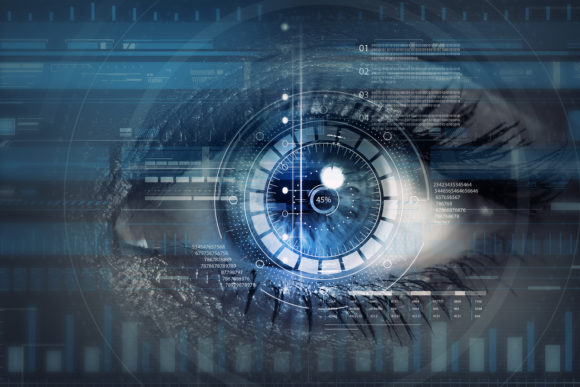
\includegraphics[scale=1]{images/cyber.jpg}
    \captionof{figure}{\textbf{Figure \arabic{figure}:} Example figure caption}
\end{center}

%Sets the bibliography style to UNSRT and imports the 
%bibliography file "samples.bib".

\bibliographystyle{unsrt}
\bibliography{Bibliographies/Phase_I_II.bib}


\listoffigures
\cleardoublepage


\end{document} 